\chapter{Un profil UML pour aider à la rédaction de GDD: \emph{Game Genesis}}
\label{chap.game-genesis}
\label{game-genesis.sect}

%GDD
Un \emph{Game Design Document}, tel que décrit à la Section~\ref{sect.GDD}, permet de réunir toutes les informations de design nécessaires au développement d'un jeu vidéo. La structure du GDD est définie en respectant des bonnes pratiques et selon les besoins de design du jeu concerné.


\gt{Ci-bas: il faut \^etre plus sp\'ecifique pour l'aspect Mechanics
car si tu dis <<{\bf tous} les \'el\'ements du jeu>>, alors pourquoi
faudrait-il autre chose que cela!?}

%MDA
Le \emph{Framework Mechanics, Dynamics, Aesthetics}, décrit au Chapitre~\ref{chap.MDA}, permet de séparer les différents aspects du design d'un jeu vidéo. L'aspect \emph{Mechanics} permet de représenter les éléments du jeu rattachés aux données et aux algorithmes, l'aspect \emph{Dynamics} décrit le comportement des \'el\'ements de \emph{Mechanics}, alors que l'aspect \emph{Aesthetics} d\'ecrit les émotions découlant de la \emph{Dynamics} que le jeu génère chez le joueur.

%UML
Les profils UML, décrits au Chapitre~\ref{chap.profils-UML}, permettent d'étendre les concepts présents dans UML. Mettre en place un profil UML permet de faciliter la cr\'eation d'un modèle et de son contenu pour un domaine particulier. Un profil se compose de stéréotypes, de valeurs étiquetées et de contraintes, qui ensemble permettent de d\'efinir de nouveaux concepts utilisables dans la description de modèles.


\section{Un aper\c{c}u de \emph{Game Genesis}}
\label{sect.gg_what}
%quoi
\emph{Game Genesis} est un profil UML que nous avons d\'evelopp\'e et qui permet d'adapter UML au domaine du design de jeux vidéos. 
Plus précisément, \emph{Game Genesis} introduit de nouvelles classes et associations --- par le biais de st\'er\'eotypes --- afin de décrire les {\bf éléments de \emph{Mechanics}} d'un GDD.

\begin{comment}
\GT{J'ai mis ici la partie ci-bas (2 paragraphes), qui était
auparavant à la fin de la section, car sinon ça semblait
redondant. Par contre, je me demande si elle ne devrait pas simplement
être supprimé, car elle semble simplement répéter ce qui a été dit à
la fin du chapitre précédent, non? Il me semble que oui, donc je mets
en commentaire: à vérifier si tu es d'accord.}

%pourquoi
L'utilisation de diagrammes de classes UML apporte certains avantages pour la modélisation des \'el\'ements de \emph{Mechanics}:
\begin{itemize}
    \item Structure;
    \item Langage de modélisation formel et normalisé;
    \item Support de communication visuel; \gt{Pas trop certain de ce que cela veut dire, i.e., un peu vague: <<performant>>!}
    \item Facilement versionnable
    \item Assez souple pour s'adapter aux domaines ou aux plateformes de développement; \gt{s'adapter \`a quoi!?}
    \item Utilisation d'outils adaptés.
\end{itemize}

Cependant, UML est un langage avant tout destiné à modéliser les systèmes informatiques et les processus d'affaire. 
Il est donc nécessaire de l'adapter afin de lui apporter le vocabulaire et les logiques nécessaires à la description de l'aspect \emph{Mechanics} d'un jeu vidéo.
C'est à cela que sert le profil \emph{Game Genesis}.
   
\GT{Fin de la partie déplacée, qui devrait probablement être supprimée, non?}
\end{comment}

\gt{Ci-bas et ailleurs. Je ne crois pas que tu devrais utiliser
directement le terme Mechanics comme dans <<un certain nombre de
Mechanics>>.  Comme indiqu\'e pr\'ec\'edemment (vieille remarque GT),
il me semble que Mechanics, en anglais, est plus compris au sens de
<<la m\'ecanique>> --- m\'ecanique des fluides, m\'ecanique quantique,
etc.  C'est pour cela que, plus haut, j'ai chang\'e pour <<l'aspect
Mechanics>>, que ci-bas j'ai indiqu\'e <<\'el\'ements de Mechanics>>.}

\gt{Et je viens de regarder l'article initial sur MDA.  L\`a aussi,
les termes Mechanics, Dynamics et Aesthetics sont consid\'er\'es comme
des substantifs au singulier: <<Mechanics describes the particular
components of the game, ...>>, <<Dynamics describes the run-time
behavior...>>, <<Aesthetics describes...>>.}


\gt{Et le terme <<aspect>> me semble aussi appropri\'e --- bien que
celui de <<vue>> ou <<point de vue>> pourrait aussi l'\^etre: <<Each
component of the MDA framework can be thought of as a 'lens' or a
'view' of the game...>>.}



Afin de rédiger un GDD, un \emph{game designer} doit d'abord définir les bases du jeu.
Durant cette étape, le \emph{game designer} va devoir définir un certain nombre d'\'el\'ements de \emph{Mechanics} qui correspondent aux objets présents dans le jeu ainsi que leurs actions et interactions.
Ces \'el\'ements de \emph{Mechanics} peuvent aussi bien être des objets visibles dans le jeu --- comme des personnages, des ennemis, des armes, des bâtiments --- mais également des \'el\'ements autour du jeu --- comme des cartes, des chronomètres, des statistiques, etc.
Tous ces \'el\'ements de \emph{Mechanics} ont des caractéristiques qui leur sont propres.

\begin{figure}[H]
    \begin{adjustbox}{width=\linewidth}
        \begin{forest}
         [\texttt{GameGenesis}
         [\texttt{Item}
             [\texttt{Wearable},tier=2
                 [\texttt{Weapon},tier=before
                    [Fig.~\ref{A-Weapon},tier=bottom]
                 ]
                 [\texttt{Equipment},tier=before
                    [Fig.~\ref{A-Equipment},tier=bottom]
                 ]
                 [\texttt{Jewerly},tier=before
                    [Fig.~\ref{A-Jewerly},tier=bottom]
                 ]
                 [\texttt{Tool},tier=before
                    [Fig.~\ref{A-Tool},tier=bottom]
                 ]
             ]
             [\texttt{AddOn},tier=2
                    [Fig.~\ref{A-Add-on},tier=bottom]
             ]
             [\texttt{Usable},tier=2
                    [Fig.~\ref{A-Usable},tier=bottom]
             ]
             [\texttt{Craft},tier=2
                    [Fig.~\ref{A-Craft},tier=bottom]
            ]
             [\texttt{Currency},tier=2
                    [Fig.~\ref{A-Currency},tier=bottom]
            ]
         ]
         ]
        \end{forest}
    \end{adjustbox}
    \caption{L'arbre des stéréotypes de \emph{Game Genesis}.}
    \label{fig.GG}
    \label{fig.GG1}
\end{figure}
    
\begin{figure}[H]
    \begin{adjustbox}{width=\linewidth}
        \begin{forest}
         [\texttt{GameGenesis}
         [\texttt{Animate} ,tier=2
                [Fig.\ref{A-Animate},tier=bottom]
         ]
         [\texttt{CharacterSheet},tier=2
                [\texttt{Statistic},tier=before
                    [Fig.~\ref{A-Statistic},tier=bottom]
                ]
                [\texttt{Attribute},tier=before
                    [Fig.~\ref{A-Attribute},tier=bottom]
                ]
                [\texttt{Information},tier=before
                    [Fig.~\ref{A-Information},tier=bottom]
                ]
                [\texttt{Experience},tier=before]
                [\texttt{Ability},tier=before]
                [\texttt{Ranking},tier=before]
         ]
         [\texttt{Lore} ,tier=2
                [Fig.~\ref{A-Lore},tier=bottom]
         ]
         [\texttt{World} ,tier=2
                [Fig.~\ref{A-World},tier=bottom]
         ]
         [\texttt{Interaction},tier=2
                [Fig.~\ref{A-Interaction},tier=bottom]
         ]
         ]
        \end{forest}
    \end{adjustbox}
    \caption{L'arbre des stéréotypes de \emph{Game Genesis} (suite).}
    \label{fig.GG2}
\end{figure}

%comment
\emph{Game Genesis} permet à un \emph{game designer} de répertorier et décrire ces \'el\'ements de \emph{Mechanics} sous forme de diagrammes de classes.
Chaque catégorie de \emph{Mechanics} est représentée par une classe, et
chaque \'el\'ement de \emph{Mechanics} est aussi représenté par une classe.
L'appartenance à une catégorie est définie par des relations d'héritage.
Les caractéristiques des catégories et des divers \'el\'ements de \emph{Mechanics} sont représentées par des attributs.
Finalement, certaines interactions entre \'el\'ements du jeu peuvent être représentées par des associations entre classes, associations auxquelles peuvent être associ\'ees certaines contraintes.

Les figures~\ref{fig.GG} et~\ref{fig.GG2} présentent une vue d'ensemble des différents stéréotypes introduits par \emph{Game Genesis} --- seuls les niveaux supérieurs de la hiérarchie des stéréotypes sont indiqués.



\goodbreak

\section{\emph{Game Genesis} en détail}

\begin{samepage}
Dans les sous-sections qui suivent, nous définissons plus en détail les éléments suivants de \emph{Game Genesis}~: 
\begin{itemize}
    \item Les stéréotypes qui permettent d'étendre les classes.
    \item Les stéréotypes qui permettent d'étendre les associations.
    \item Les contraintes qui d\'efinissent des règles d'utilisation des stéréotypes.
\end{itemize}
\end{samepage}

\subsection{Les stéréotypes}

\gt{Dans la figure, comme ce sont des \'el\'ements de <<code>> ---
classes UML --- il vaut mieux utiliser la police teletype.}

\gt{Ce serait pr\'ef\'erable que dans les deux parties de la figure,
les r\'ef\'erences aux annexes soient pr\'esent\'ees de la m\^eme
fa\c{c}on pouar Animate, Lore, World et Interaction. Sinon, cela donne
l'impression que la s\'emantique pourrait \^etre diff\'erente ---
parce que c'est bien la m\^eme, n'est-ce pas?}


\begin{figure}
    \centering
    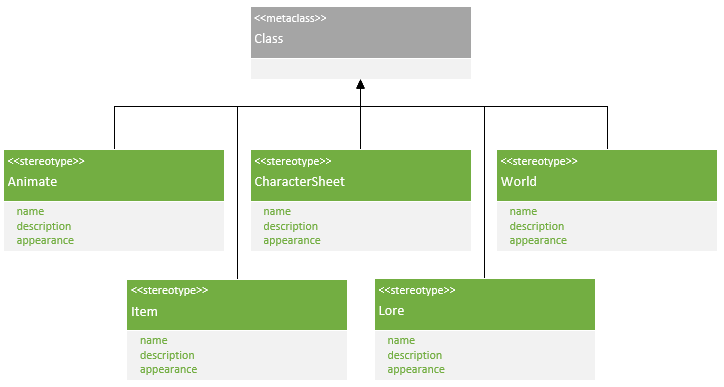
\includegraphics[width=\linewidth]{10_img/chap5/metaclass_class.PNG} 
    \caption{La spécification de certains stéréotypes de \emph{Game Genesis}, obtenus par \emph{extension} de la m\'etaclasse \texttt{Class}.}
    \label{fig.meta_class}
\end{figure}

\gt{Ci-bas: dans le cas pr\'esent, ce n'est pas tant une
<<red\'efinition>> qu'une extension, qu'une cr\'eation de nouvelles
classes, de nouveaux concepts! Donc, j'ai modifi\'e en cons\'equence.}

Dans la section~\ref{sect.uml.ster}, nous avons décrit le mécanisme d'extension de m\'etaclasses afin d'introduire de nouveaux concepts par le biais de stéréotypes. 
Dans \emph{Game Genesis}, nous faisons donc usage des stéréotypes afin d'étendre les classes d'un modèle de jeu et ainsi permettre la rédaction de GDD.
%
Les racines des arbres définissant ces divers stéréotypes sont
présentées aux figures~\ref{fig.GG} et~\ref{fig.GG2}, alors que les
détails des sous-arbres sont présentés en annexe, dans une figure
dont le numéro est indiqué sur ces figures.

La figure~\ref{fig.meta_class} présente les différentes <<~racines~>> de \emph{Game Genesis}. 
Ce sont les premiers stéréotypes du profil qui serviront majoritairement de catégories de haut niveau pour classifier les éléments de \emph{Mechanics} décrits dans un \emph{Game Design Document}.
Nous présentons le profil plus en détail dans l'Annexe~\ref{AnnexeA}.
%
Comme on le remarque, ces stéréotypes sont des \emph{extensions} de la
métaclasse \texttt{Class}, donc ils serviront à annoter des classes, des concepts.


Dans un article de Salazar \emph{et al.}~\cite{GDD_software}, plus particulièrement dans la documentation additionnelle de cet article~\cite{salazar_gdd}, nous avons identifié un certain nombre d'\'el\'ements de \emph{Mechanics} typiquement présents dans un GDD.
Nous avons constaté que les éléments étaient répartis dans des catégories possédant elles-mêmes certaines caractéristiques communes. 
Nous avons ainsi extrait les catégories suivantes :

\begin{itemize}
    \item \emph{Player Character}
    \item \emph{Non Player Character}
    \item \emph{Enemy}
    \item \emph{Final Enemy}
    \item \emph{Help Object}
    \item \emph{Extra Object}
    \item \emph{Other Object}
\end{itemize}


\gt{J'ai oté <<très larges>> car <<très larges et spécifiques>> me semblait contradictoire!}

Ces catégories sont cependant plutôt spécifiques au jeu décrit dans cet exemple de \emph{Game Design Document}, à savoir \emph{Donkey Kong}~\cite{salazar_gdd}.
Donc, ces catégories ne permettent pas forcément de représenter les éléments de \emph{Mechanics} de jeux différents de \emph{Donkey Kong}.
Par la suite, nous avons essayé de définir des catégories et des éléments en fonction de différents \emph{Game Design Documents} et de notre expérience personnelle de l'utilisation des jeux vidéos.
Nous avons alors défini les stéréotypes présents dans les figures~\ref{fig.GG1} et~\ref{fig.GG2},
figures qui renvoient vers une modélisation plus en détail présentée dans l'Annexe~\ref{AnnexeA}.

\gt{Ci-haut: il faut expliquer pourquoi ces catégories que tu
identifies ne se retrouvent pas dans les figures 5.1 et 5.2 --- donc
expliquer (?) qu'elles correspondent à des détails de l'annexe (?).}

\gt{Ci-haut: Si ce sont des noms de classes, pr\'esents dans le
mod\`ele/profil UML, alors il faut utiliser la convention des noms de
classe UML, i.e., un seul <<mot>> en CamelCase: PlayerCharacter,
FinalEnemy, etc.}
\eh{J'ai enlevé le txt teletype dans cet itemize car ce sont des éléments présents dans l'exemple de GDD Donkey Kong de l'article (sous forme textuel) et non pas des éléments du profil qui sont cités}

\gt{Par contre, comme ce sont des termes en anglais, il vaut mieux les
mettre en italiques.}

Les classes UML fonctionnant avec un système d'héritage,
un \'el\'ement de \emph{Mechanics} hérite donc des attributs énoncés dans les catégories parentes.
\begin{comment}
Phrase inutile!
C'est ainsi que nous avons décidé d'utiliser un diagramme de classes afin de représenter les \'el\'ements de \emph{Mechanics} comme des classes et de spécifier leurs caractéristiques dans les attributs.
\end{comment}
%
\gt{Je crois que les phrases qui suivent sont redondantes, n'apportent
rien de plus. Sinon, il faut les reformuler, car je ne comprends pas
bien ce qu'elles introduisent de nouveau.}
\eh{Supprimées}

\begin{figure}
    \centering
    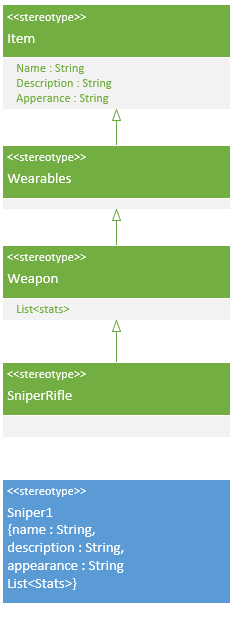
\includegraphics[width=5cm]{10_img/chap5/sniper2.PNG} 
    \caption{Une classe \texttt{Sniper1} utilisant le stéréotype
    \texttt{SniperRifle}, et donc qui h\'erite des attributs (directs et indirects) associ\'es à son stéréotype \texttt{SniperRifle}.}
    \label{fig.sniper}
\end{figure}

\gt{Idem pour ce qui suit!}
%

\gt{Dans la figure 5.4, boite pour Sniper1. a. Changer <<stereotype>>
par <<SniperRifle>>. b. Il devrait y avoir une ligne (sous-boite de
couleur différente?) qui sépare le nom de la classe de liste des
attributs.}

La figure~\ref{fig.sniper} pr\'esente un exemple d'une classe \texttt{Sniper1}, un élément de \emph{Mechanics} d'un GDD pour un jeu qui serait d\'efini avec le profil \emph{Game Genesis}.
La classe \texttt{Sniper1} est stéréotypée avec \texttt{SniperRifle}, donc elle
hérite des attributs des divers stéréotypes de la hiérarchie d'héritage de classes.
Une instance de la classe \texttt{Sniper1} possèdera donc les attributs des stéréotypes \texttt{Item}, \texttt{Wearable}, \texttt{Weapon} et \texttt{SniperRifle}.

\gt{Ci-haut et dans la figure: non, ce n'est pas ainsi qu'il faut
pr\'esenter cela il me semble. Plusieurs remarques. 1) Ce serait bien
de toujours distinguer, par les couleurs, la sp\'ecification du profil
(bleu!) de son utilisation (vert!). Or, la sp\'ecification de Sniper1
est une utilisation.  2) Si tu mets directement les d\'etails dans la
boite Sniper1, alors c'est comme si l'usager les sp\'ecifiait
lui-m\^eme. Or, ici, de ce que je comprends, tu essaies d'expliquer
qu'il y a h\'eritage implicite.  Une possibilit\'e serait de mettre en
vert une boite avec <<SR>> et Sniper, sans attributs, puis juste \`a
cot\'e de mettre une boite (autre couleur?) avec juste Sniper comme
nom mais o\`u tous les attributs sont maintenant pr\'esents ---
justement \`a cause de l'h\'eritage {\bf implicite} associ\'e \`a ta
hi\'erarchie de st\'er\'eotypes.}

\gt{En d'autres mots, il me semble que tu dois insister plus sur le
fait que la sp\'ecification d'un st\'er\'eotype introduit un nouveau
{\bf concept} --- une nouvelle classe ---, lequel concept peut
\'evidemment poss\'eder des attributs --- indiqu\'es directement (dans
sa boite) ou indirectement (via h\'eritage).  Une fois ce concept
d\'efini, on peut ensuite l'utiliser pour d\'efinir de nouvelles
classes, dont les objets poss\`edent tous les attributs associ\'es au
concept --- peu importe d'o\`u proviennent ces attributs (directs ou
indirects).}

\gt{De plus, puisque tu as un exemple d'utilisation du st\'er\'eotype
SR, tu devrais aussi donner un exemple de sp\'ecification/utilisation
des valeurs \'etiquet\'ees pour sp\'ecifier des attributs.}



\subsection{Les interactions}

\begin{figure}
    \centering
    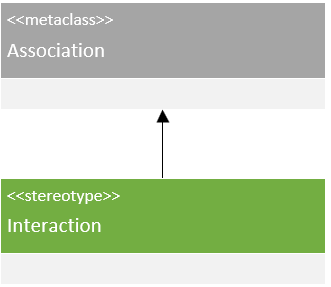
\includegraphics[width=5cm]{10_img/chap5/metaclass_association.PNG} 
    \caption{La spécification du stéréotype \texttt{Interaction} de \emph{Game Genesis}, obtenu par \emph{extension} de la m\'etaclasse \texttt{Association}.}
    \label{fig.meta_assoc}
\end{figure}

Les éléments de \emph{Mechanics} ne sont pas tous des éléments isolés et une expérience de jeu ne serait rien sans les interactions que le joueur peut avoir avec les divers \'el\'ements du jeu.

La Figure~\ref{fig.meta_assoc} représente la spécification des stéréotypes présents dans la catégorie \texttt{Interaction}.
Contrairement aux autres stéréotypes du profil \emph{Game Genesis} qui étendent les classes, celui d'\texttt{Interaction} étend plutôt la métaclasse \texttt{Association}.

\begin{table}
\begin{center}
\begin{tabular}{|l|l|}\hline
\texttt{Use} &
\texttt{Drop}
\\\hline
\texttt{Move}&
\texttt{Destroy}
\\\hline
\texttt{Trade} &
\texttt{Stack}
\\\hline
\texttt{Attach}&
\texttt{Attack}
\\\hline
\texttt{Wear}&
\\\hline
\end{tabular}
\end{center}
\caption{Les interactions de Salazar \emph{et al.}~\cite{salazar_gdd} intégrées dans \emph{Game Genesis}.}
\label{table.interactions}
\end{table}


Des interactions fréquemment rencontrées sont présentées dans le gabarit de GDD de Salazar \emph{et al.}~\cite{salazar_gdd}, qui les présente sous forme de règles d'interaction.
Ces règles sont composées de divers éléments, dont les suivants :
\begin{itemize}
    \item Deux \'el\'ements (ou plus) de \emph{Mechanics};
    \item Une interaction entre ces \'el\'ements;
    \item Une contrainte appliquée à cette interaction (optionnelle).
\end{itemize}
Les interactions de Salazar \emph{et al.} que nous avons intégrées à \emph{Game Genesis} sont présentées dans le tableau~\ref{table.interactions} --- voir aussi la Figure~\ref{A-Interaction}.


\gt{Il faut aussi que tu montres clairement, parce que c'est dans le
contexte d'un profil UML, qu'il s'agit d'extension de la Metaclass
fAssociation d'UML --- comme \'evoqu\'e l'autre fois (quand on s'est
rencontr\'es? je ne suis plus certain.}

\gt{Idem pour les st\'er\'eotypes de classes de la section
pr\'ec\'edente: on devrait voir ici -- et possiblement aussi dans
l'annexe --- qu'il s'agit d'extension de la Metaclass Class!}

\subsection{Quelques contraintes}

Dans un profil UML, il est fréquent d'imposer des contraintes d'utilisation sur les \'el\'ements du profil afin de le rendre plus précis et d'éviter des problèmes de compréhension ou d'incohérence du modèle.
Dans \emph{Game Genesis}, il est difficile d'établir un grand nombre de contraintes, le profil devant s'appliquer à de nombreux types de mécaniques de jeu.
\begin{comment}
Je ne comprends pas trop cette phrase
C'est en essayant de laisser assez de liberté aux \emph{game designers} que certaines contraintes ne peuvent pas être appliquées ou sont situationnelles.
\end{comment}

Voici quand m\^eme une br\`eve liste de contraintes envisageables dans un profil tel que \emph{Game Genesis} :
\begin{itemize}
    \item Une interaction entre \texttt{Player} et \texttt{Weapon} ne peut être que \texttt{Grab} ou \texttt{Equip};
    \item Une interaction entre \texttt{Player} et \texttt{Equipment} ne peut être que \texttt{Grab} ou \texttt{Equip};
    \item Une interaction entre \texttt{AddOn} et \texttt{Weapon} ou \texttt{Equipment} ne peut être que \texttt{Attach};
\end{itemize}

\gt{Je ne comprends pas la contrainte sur AddOn~:(} 

Certaines contraintes peuvent être situationnelles comme celles ci-dessous :
\begin{itemize}
    \item Si le jeu est \texttt{PvP} (\emph{Player versus Player}) alors \texttt{Player} \texttt{<<attack>>} \texttt{Player} est possible,
    \item Si le jeu n'est pas \texttt{PvP} alors \texttt{Player} \texttt{<<attack>>} \texttt{Player} n'est pas possible.
\end{itemize}


\gt{Ci-haut: dans ce cas, si tu comptes \'enoncer une telle
contrainte, il faudrait que ton profil inclut un attribut qui permet
d'indiquer si le jeu et PvP ou non.}
\eh{Un tel attribut serait trop contraignant dans le cadre d'une conception de jeux. Certains jeux sont PVP, d'autres PVE, d'autres ont des zones uniquement PVP et/ou PVE, certains crééent plusieurs serveurs qui sont soit PVP soit PVE, etc.
Le PVP ou PVE sont des mécaniques de gameplay }

\section{Conclusion}
%
%\GT{Dire que tu as <<réussi>> est trop fort!}
%
Dans ce chapitre, nous avons tenté d'exprimer les concepts de base d'un profil UML pour la rédaction d'un \emph{Game Design Document}.
Dans son état actuel, ce profil, \emph{Game Genesis}, est cependant plus une <<preuve de concept>> qu'une version complète qui pourrait couvrir tous les besoin d'un \emph{game designer}.
\emph{Game Genesis} est incomplet car :
\begin{itemize}
    \item seuls les aspects \emph{Mechanics} sont traités;
    \item les catégories sont non exhaustives;
    \item le profil est spécifié de façon non formelle, aucun outil UML <<officiel>> n'ayant été utilisé pour le spécifier.
\end{itemize}

Il serait quand même intéressant de voir comment \emph{Game Genesis} peut être utilisé dans le cadre de la rédaction d'un \emph{Game Design Document} pour un jeu existant.
C'est ce que nous faisons dans le prochain chapitre.




%%%%%%%%%%%%%%%%%%%%%%%%%%%%%%%%%%%%%%%%%%%%%%%%%%%%%%%%%%%%%%%%%%%%%%%%%%
\begin{comment}
\chapter{Un langage de modélisation pour l'établissement d'un Game Design Document}

\section{Le concept}
\subsection{Définition}
\subsubsection{Quoi ?}
Un langage permettant de modéliser et stocker des idées lors des phases de Breakthrough et de Conception d'un projet de jeu vidéo. La modélisation peut être graphique et/ou textuelle avec application des modifications en parallèle. \\
Les informations peuvent contenir tout le nécessaire pour exprimer les idées (textes, informations numériques, chemins de fichiers...). Les champs peuvent être personalisables pour permettre de la souplesse aux utilisateurs.

\subsubsection{Pour quoi faire ?}
\paragraph{Des outils de modélisation existent pour tous les domaines reliés au développement de logiciels. Ils sont souvent spécifiques à un corps de métier afin de pouvoir proposer un maximum de fonctionnalités spécifiques sans devenir trop compliqué et en utilisant un vocabulaire précis qui correspond au corps de métier concerné.}

\paragraph{Il y a peu ou pas de langages de modélisation plus généraux pour des domaines multi-métiers. Le but est de pouvoir modéliser la réflexion créative en fournissant un élément visuel permettant de mind-mapper les idées, les stocker et les réutiliser. \\
Il faut que la modélisation soit assez souple pour pouvoir répondre aux besoins de chacun des corps de métier d'où le fait que les éléments et attributs peuvent avoir des identifiants spécifiques définis librement par l'utilisateur.}

\subsubsection{Pour quelles raisons ?}
\paragraph{Les supports de réflexion actuellement utilisés : cahier des charges, réunions, notes écrites, mails, minds-maps... L'organisation de ces différents supports dans un ensemble cohérent est tr;s compliqué. Dans un cahier des charges il est compliqué de classer les idées à la volée. Un mind-map nécessite une numérisation ou une retranscription sur un outil de mind-mapping qui sont toutes les deux des techniques non péreines et risquées dans la conservation des données. Des notes écrites peuvent se perdre et n'ont pas de durabilité sur le long terme. Des mails sont péreins mais il est difficile de les organiser pour le stockage de l'information.}
\paragraph{Un langage de modélisation graphique et textuel permettrait de mind-mapper les idées à la volée sous forme de cubes contenant les données nécessaires. La hiérarchisation des éléments permettrait de gérer des héritages et des relations ainsi que d'éviter la répétition trop abondante des mêmes informations. Les faces des cubes permettrait d'isoler les informations nécessaires à chacun des corps de métier.}
\end{comment}


